\section{分支变化}
\label{sec:sens-branches}

上一节的局部导数有前提。前提不成立时，导数为什么会失效，失效的方式有什么不同？本节用三个能够手算的例子回答。活动集改变时，可用的方程变了。全局最优解切换时，所选的分支变了。方程退化时，线性方程不再可逆。三种情况的数学原因不同，都不是某个算法的不稳定。

\subsection{活动集改变}
\label{sec:sens-active-change}

\paragraph{分段解出预算例}
把预算例按活动集分成三段，每段都用KKT条件解出。

当$\tau>3$时，理想点$(2,1)$满足$x_1+x_2\leq\tau$，全部约束不起作用：
\[
 \bm{x}^\star=(2,1),\qquad\bm{\lambda}=\bm{0},\qquad V(\tau)=0.
\]

当$1<\tau<3$时，只有预算起作用。平稳条件是$x_1-2+\lambda_1=0$、$x_2-1+\lambda_1=0$，代入$x_1+x_2=\tau$，得到$3-2\lambda_1=\tau$，于是
\[
 \lambda_1=\frac{3-\tau}{2},\qquad
 \bm{x}^\star=\Bigl(\frac{\tau+1}{2},\ \frac{\tau-1}{2}\Bigr).
\]
两个坐标与乘子在这段都是正的。目标值是$\lambda_1^2$，即$V(\tau)=(3-\tau)^2/4$。

当$0<\tau<1$时，预算和$x_2\geq0$起作用，$\bm{x}^\star=(\tau,0)$。平稳条件的两个分量是$x_1-2+\lambda_1=0$和$x_2-1+\lambda_1-\lambda_3=0$，由此解出
\[
 \lambda_1=2-\tau,\qquad\lambda_3=1-\tau.
\]
两者都为正。目标值是
\[
 V(\tau)=\frac12(2-\tau)^2+\frac12.
\]

\begin{BookInlineTable}
 \centering
 \begin{tabular}{cccc}
  \toprule
  区间 & $\bm{x}^\star(\tau)$ & $(\lambda_1,\lambda_3)$ & $V'(\tau)$\\
  \midrule
  $0<\tau<1$ & $(\tau,\ 0)$ & $(2-\tau,\ 1-\tau)$ & $\tau-2$\\
  $1<\tau<3$ & $\bigl(\frac{\tau+1}{2},\ \frac{\tau-1}{2}\bigr)$ & $\bigl(\frac{3-\tau}{2},\ 0\bigr)$ & $\frac{\tau-3}{2}$\\
  $\tau>3$ & $(2,\ 1)$ & $(0,\ 0)$ & $0$\\
  \bottomrule
 \end{tabular}
 \caption{预算例的三段解，$\lambda_2$在所有区间都等于零。每一段内$V'(\tau)=-\lambda_1$，这正是乘子的边际解释。}
 \label{tab:sens-budget-pieces}
\end{BookInlineTable}

\paragraph{连接点上发生了什么}
图~\ref{fig:sens-activeset-path}画出解在平面上的路径，图~\ref{fig:sens-activeset-curves}画出各个量随$\tau$的变化。解的路径是一条折线，在$\tau=1$与$\tau=3$处转弯。

\begin{BookInlineFigure}
 \centering
 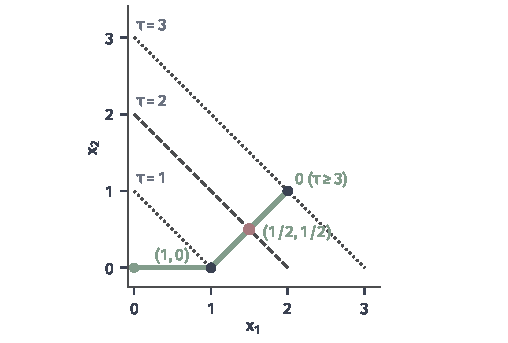
\includegraphics[width=86mm]{figures/05-optimization/06-constrained-optimization/matplotlib/sens-activeset-path/figure.pdf}
 \caption{最优解$\bm{x}^\star(\tau)$在平面上的路径（绿线）。虚线与点线是几条预算线，黑点是活动集改变的位置，红点是$\tau=2$的解。绿色文字是各段上解对$\tau$的导数：第一段$(1,0)$，第二段$(1/2,1/2)$，$\tau\geq3$时为零。}
 \label{fig:sens-activeset-path}
\end{BookInlineFigure}

$\tau=1$处，$x_2\geq0$刚要失去作用，$\lambda_3=0$。$\tau=3$处，预算刚要失去作用，$\lambda_1=0$。两处都有活动约束的乘子等于零，严格互补恰好在连接点失败。

解在连接点连续但不可微。$\tau=1$处的左导数和右导数分别是
\[
 \bm{x}'(1^-)=(1,0),\qquad\bm{x}'(1^+)=\Bigl(\frac12,\frac12\Bigr).
\]
值函数却不一样。两段的$V'$在$\tau=1$处都等于$-1$，在$\tau=3$处都等于$0$，所以$V$在连接点可微，只是二阶导数有跳跃。原因是$V'=-\lambda_1$，而$\lambda_1$连续穿过连接点：进入或离开活动集的约束，它的乘子在那里恰好是零，不造成$\lambda_1$的跳变。

\begin{BookInlineFigure}
 \centering
 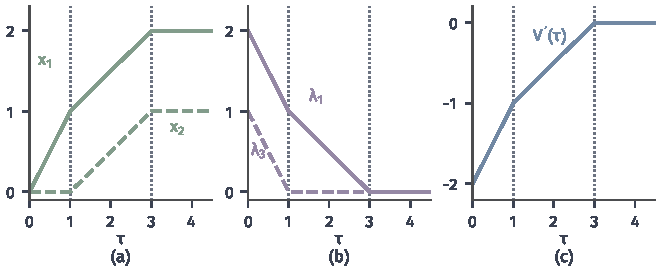
\includegraphics[width=112mm]{figures/05-optimization/06-constrained-optimization/matplotlib/sens-activeset-curves/figure.pdf}
 \caption{预算例各量随$\tau$的变化，灰色点线标出$\tau=1,3$。(a)~解的两个分量（实线$x_1$，虚线$x_2$）在连接点转折。(b)~乘子$\lambda_1$（实线）、$\lambda_3$（虚线）连续，但斜率改变。(c)~$V'(\tau)$连续，说明$V$在连接点仍然可微。}
 \label{fig:sens-activeset-curves}
\end{BookInlineFigure}

\paragraph{固定活动集的公式不能外推}
公式必须限定在它的区间内使用。把活动集$\{1\}$的公式用到$\tau=0.5$，得到$x_2=-0.25$，不可行。用到$\tau=4$，得到$\lambda_1=-1/2$，乘子符号错误。这两种错误恰好给出判别方法：预测的不活动约束是否越界，预测的乘子是否变负。

连接点上只有单侧的导数。向哪一侧走，就要换用那一侧的活动集重新写方程，上面的$\bm{x}'(1^-)$和$\bm{x}'(1^+)$正是这样得到的。

\subsection{全局最优解切换}
\label{sec:sens-global-switch}

\paragraph{两个候选的比较}
活动集改变时解连续地走过连接点。全局最优解还可能在两个相距很远的候选之间跳动。最简单的例子是在两点集合上选最小：
\begin{equation}
 \min_{x\in\{-1,1\}}\ \theta x.
 \label{eq:sens-two-points}
\end{equation}
把两个候选分别看成两条分支：
\[
 x=1:\quad v_1(\theta)=\theta,\qquad\qquad
 x=-1:\quad v_2(\theta)=-\theta.
\]
每条分支上解都是常数，$\bm{x}'=0$，值是线性函数，两者都光滑。

全局最优值取两条分支的较小者，最优解集合随$\theta$的符号改变：
\begin{equation}
 V(\theta)=-\lvert\theta\rvert,\qquad
 \bm{S}(\theta)=\begin{cases}\{1\},&\theta<0,\\\{-1,1\},&\theta=0,\\\{-1\},&\theta>0.\end{cases}
 \label{eq:sens-switching}
\end{equation}

图~\ref{fig:sens-switching}分别显示了三件事。每条分支在$\theta=0$处都很光滑。全局值在$\theta=0$处不可微。解集合在$\theta=0$处从一个点变成两个点，再变回另一个点，选出的解不连续。

\begin{BookInlineFigure}
 \centering
 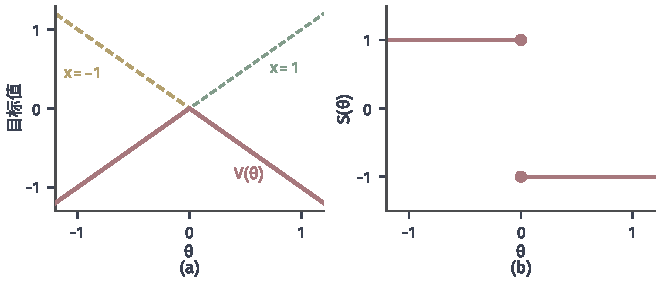
\includegraphics[width=112mm]{figures/05-optimization/06-constrained-optimization/matplotlib/sens-switching/figure.pdf}
 \caption{在$\{-1,1\}$上最小化$\theta x$。(a)~绿色虚线是$x=1$分支的值，黄色虚线是$x=-1$分支的值，红线是全局最优值$-\lvert\theta\rvert$。(b)~全局最优解集合，$\theta=0$处两个点都最优，解在此跳跃。}
 \label{fig:sens-switching}
\end{BookInlineFigure}

\paragraph{三个对象分别的结论}
定理~\ref{thm:sens-danskin}在这里成立：$\bm{C}=\{-1,1\}$是紧集，$\partial f/\partial\theta=x$连续。在$\theta=0$处，它给出
\[
 V'(0;d)=\min_{x\in\{-1,1\}}xd=-\lvert d\rvert,
\]
这与$V(\theta)=-\lvert\theta\rvert$一致。

把一条分支的导数推广成全局公式是常见的错误。$x=1$分支的导数在$\theta>0$时仍然是$1$，但$\theta>0$时全局最优解已经是$-1$，全局值的导数是$-1$。第~\ref{sec:sens-problems}节的双谷目标在连续变量上重现了同样的现象：每个谷底都有光滑的分支，全局最优解在$\theta=0$处跳到另一个谷底。在双谷的右侧分支上，驻点方程$4x^3-4x+\theta=0$对$x$的导数在$x=1$处是$8$，隐函数定理给出
\[
 x'(0)=-\frac{1}{8}.
\]
这个导数描述的是右侧谷底的移动，与全局最优解在$\theta=0$处的跳跃无关。

\subsection{退化与变化尺度}
\label{sec:sens-degeneracy}

前两种失效换了方程或换了分支。第三种失效中方程和分支都没有换，解甚至唯一，只是线性化之后的方程退化了。

\paragraph{唯一解也可能没有有限导数}
考虑
\begin{equation}
 \min_{x\in\mathbb{R}}\ \frac14x^4-\theta x.
 \label{eq:sens-quartic}
\end{equation}
对每个$\theta$，目标严格凸且强制，最优解唯一。驻点方程$x^3=\theta$给出
\[
 x^\star(\theta)=\theta^{1/3}.
\]

$\theta=0$处$x^\star=0$，Hessian$3x^2$等于零，隐函数定理的条件不成立。真实导数是
\[
 \frac{\mathrm{d}x^\star}{\mathrm{d}\theta}=\frac{1}{3\theta^{2/3}}\quad(\theta\neq0),
\]
$\theta\to0$时趋于$+\infty$，解函数在$\theta=0$处有竖直的切线。参数变化$10^{-6}$，解移动$10^{-2}$，一万倍的放大，见图~\ref{fig:sens-quartic}(b)。

值函数却没有这个问题。把解代入，
\[
 V(\theta)=\frac14\theta^{4/3}-\theta^{4/3}=-\frac34\lvert\theta\rvert^{4/3},
\]
并且$V'(\theta)=-\theta^{1/3}$，在$\theta=0$处等于零。这正是包络关系：$\partial f/\partial\theta=-x$，只需知道解的位置，不需要它的导数。再一次看到，值比解更稳定。

\begin{BookInlineFigure}
 \centering
 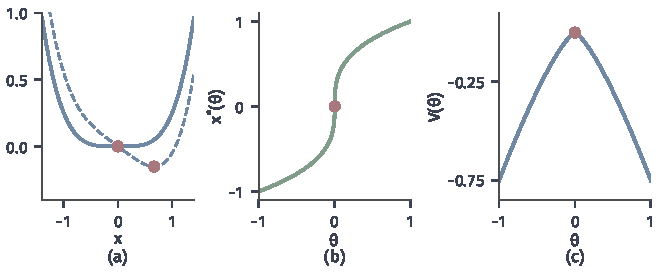
\includegraphics[width=112mm]{figures/05-optimization/06-constrained-optimization/matplotlib/sens-quartic/figure.pdf}
 \caption{退化的唯一最优解。(a)~目标$x^4/4-\theta x$，实线$\theta=0$，虚线$\theta=0.3$，红点是最小点。$\theta=0$时谷底二阶平坦。(b)~最优解$\theta^{1/3}$在$\theta=0$处切线竖直。(c)~最优值$-\tfrac34\lvert\theta\rvert^{4/3}$在$\theta=0$处可微。}
 \label{fig:sens-quartic}
\end{BookInlineFigure}

\paragraph{非退化时的放大倍数}
矩阵$\bm{K}$可逆但接近奇异时，导数存在却很大。记$\bm{z}=(\bm{x},\bm{w})$，$\bm{B}=\bm{D}_{\bm{\theta}}\bm{F}$。由式~\eqref{eq:sens-inequality-derivative}，一阶变化满足$\bm{K}\Delta\bm{z}=-\bm{B}\Delta\bm{\theta}$，因此
\begin{equation}
 \lVert\Delta\bm{z}\rVert_2\leq\lVert\bm{K}^{-1}\rVert_2\,\lVert\bm{B}\Delta\bm{\theta}\rVert_2.
 \label{eq:sens-amplification}
\end{equation}
$\lVert\bm{K}^{-1}\rVert_2$越大，同样的参数变化引起的解和乘子的变化可能越大。下面两种几何情形都会使它变大。

第一种是约束接近平行。取两条等式约束
\[
 x_1+x_2=\tau,\qquad x_1+(1+\varepsilon)x_2=2+\varepsilon.
\]
解由它们的交点确定，$\tau=2$时交点是$(1,1)$。解线性方程，得到
\[
 \bm{x}'(\tau)=\Bigl(\frac{1+\varepsilon}{\varepsilon},\ -\frac{1}{\varepsilon}\Bigr).
\]

$\varepsilon=0.25$时导数是$(5,-4)$，$\varepsilon=0.01$时是$(101,-100)$。约束梯度仍然线性无关，LICQ成立，只是接近失效。图~\ref{fig:sens-amplification}(a)里，预算线只平移一点，交点却沿着两条线滑过很长的距离。

第二种是碗的底部很平。考虑二次目标
\[
 f(\bm{x},\bm{b})=\frac12\bm{x}^{\top}\bm{H}\bm{x}-\bm{b}^{\top}\bm{x},\qquad\bm{H}=\operatorname{diag}(1,0.1).
\]
把$b_2$从$0.1$改为$0.2$，解从$(1,1)$移到$(1,2)$。参数只变化$0.1$，解移动了$1$，放大倍数是曲率的倒数，即$10$。

\begin{BookInlineFigure}
 \centering
 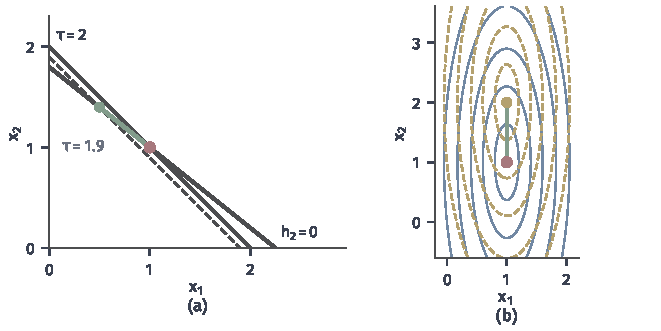
\includegraphics[width=112mm]{figures/05-optimization/06-constrained-optimization/matplotlib/sens-amplification/figure.pdf}
 \caption{两种放大机制。(a)~$\varepsilon=0.25$的两条等式约束，预算线从实线$\tau=2$平移到虚线$\tau=1.9$，交点沿绿色线段从红点移到绿点，距离约是平移量的$6.4$倍。(b)~$\bm{H}=\operatorname{diag}(1,0.1)$的目标等高线，蓝色实线是$b_2=0.1$，黄色虚线是$b_2=0.2$，最小点沿绿色线段从红点移到黄点。}
 \label{fig:sens-amplification}
\end{BookInlineFigure}

\paragraph{固有敏感性与数值误差}
上面的放大是问题的性质，与用什么算法无关。这里有两种不同的误差，需要分开。

\begin{BookInlineTable}
 \centering
 \begin{tabular}{lll}
  \toprule
  & 固有敏感性 & 数值误差\\
  \midrule
  比较 & 不同参数的精确解 & 同一问题的计算解与精确解\\
  度量 & $\bm{D}\bm{z}$的大小 & 残差、舍入与条件数\\
  改善 & 改变模型或数据 & 改进算法与精度\\
  \bottomrule
 \end{tabular}
 \caption{固有敏感性与数值误差的比较。两者都可能与$\bm{K}$的病态有关，但回答不同的问题。}
 \label{tab:sens-inherent-numerical}
\end{BookInlineTable}

矩阵的条件数大，并不一定说明解对参数敏感。把预算例中预算约束整体乘以$s>0$，写成$s(x_1+x_2-\tau)\leq0$。这是同一个约束，解不变，解对$\tau$的导数也不变，乘子则变成原来的$1/s$。相应的KKT矩阵是
\[
 \bm{K}_s=\begin{bmatrix}1&0&s\\0&1&s\\s&s&0\end{bmatrix}.
\]
$s=1$时条件数是$2$。$s=1000$时条件数约为$1415$，而$\bm{x}'(\tau)$仍然是$(1/2,1/2)$。这里的条件数变大只反映约束的书写尺度，解的敏感性没有任何变化。

解读式~\eqref{eq:sens-amplification}之前，应该先把变量和约束调整到量纲合理的尺度，计算时也应该作相应的平衡处理。只有这样，$\bm{K}$的病态才能反映问题真实的敏感性。
